\documentclass[12pt,twoside]{article}

\usepackage[backend=biber,style=alphabetic]{biblatex} 
\addbibresource{ref.bib}  


%%%%%%%%%%%%%%%%%%%%%%%%%%%%%%%%%%%%%%%%%%%%%%%%%%%%%%%%%%%%%%%%%%%%%%%%%%%%%

% Definitions for the title page
% Edit these to provide the correct information
% e.g. \newcommand{\reportauthor}{Timothy Kimber}

\newcommand{\reporttitle}{An intelligent digital interface for sharing diagnostic medical imaging with patients}
\newcommand{\reportauthor}{Laura Hagege LH}
\newcommand{\supervisor}{Fernando Bello}
\newcommand{\degreetype}{Msc. Computing Science}

%%%%%%%%%%%%%%%%%%%%%%%%%%%%%%%%%%%%%%%%%%%%%%%%%%%%%%%%%%%%%%%%%%%%%%%%%%%%%

% load some definitions and default packages
%%%%%%%%%%%%%%%%%%%%%%%%%%%%%%%%%%%%%%%%%
% University Assignment Title Page 
% LaTeX Template
% Version 1.0 (27/12/12)
%
% This template has been downloaded from:
% http://www.LaTeXTemplates.com
%
% Original author:
% WikiBooks (http://en.wikibooks.org/wiki/LaTeX/Title_Creation)
%
% License:
% CC BY-NC-SA 3.0 (http://creativecommons.org/licenses/by-nc-sa/3.0/)
% 
%
%%%%%%%%%%%%%%%%%%%%%%%%%%%%%%%%%%%%%%%%%
%----------------------------------------------------------------------------------------
%	PACKAGES AND OTHER DOCUMENT CONFIGURATIONS
%----------------------------------------------------------------------------------------
\usepackage[a4paper,hmargin=2.8cm,vmargin=2.0cm,includeheadfoot]{geometry}
\usepackage{textpos}
\usepackage{natbib} % for bibliography
\usepackage{tabularx,longtable,multirow,subfigure,caption}%hangcaption
\usepackage{fncylab} %formatting of labels
\usepackage{fancyhdr} % page layout
\usepackage{url} % URLs
\usepackage[english]{babel}
\usepackage{amsmath}
\usepackage{graphicx}
\usepackage{dsfont}
\usepackage{epstopdf} % automatically replace .eps with .pdf in graphics
\usepackage{backref} % needed for citations
\usepackage{array}
\usepackage{latexsym}
\usepackage[pdftex,pagebackref,hypertexnames=false,colorlinks]{hyperref} % provide links in pdf

\hypersetup{pdftitle={},
  pdfsubject={}, 
  pdfauthor={},
  pdfkeywords={}, 
  pdfstartview=FitH,
  pdfpagemode={UseOutlines},% None, FullScreen, UseOutlines
  bookmarksnumbered=true, bookmarksopen=true, colorlinks,
    citecolor=black,%
    filecolor=black,%
    linkcolor=black,%
    urlcolor=black}

\usepackage[all]{hypcap}


%\usepackage{color}
%\usepackage[tight,ugly]{units}
%\usepackage{float}
%\usepackage{tcolorbox}
%\usepackage[colorinlistoftodos]{todonotes}
% \usepackage{ntheorem}
% \theoremstyle{break}
% \newtheorem{lemma}{Lemma}
% \newtheorem{theorem}{Theorem}
% \newtheorem{remark}{Remark}
% \newtheorem{definition}{Definition}
% \newtheorem{proof}{Proof}


%%% Default fonts
\renewcommand*{\rmdefault}{bch}
\renewcommand*{\ttdefault}{cmtt}



%%% Default settings (page layout)
\setlength{\parindent}{0em}  % indentation of paragraph

\setlength{\headheight}{14.5pt}
\pagestyle{fancy}
\renewcommand{\chaptermark}[1]{\markboth{\chaptername\ \thechapter.\ #1}{}} 

\fancyfoot[ER,OL]{\sffamily\textbf{\thepage}}%Page no. in the left on odd pages and on right on even pages
\fancyfoot[OC,EC]{\sffamily }
\renewcommand{\headrulewidth}{0.1pt}
\renewcommand{\footrulewidth}{0.1pt}
\captionsetup{margin=10pt,font=small,labelfont=bf}


%--- chapter heading

\def\@makechapterhead#1{%
  \vspace*{10\p@}%
  {\parindent \z@ \raggedright \sffamily
    \interlinepenalty\@M
    \Huge\bfseries \thechapter \space\space #1\par\nobreak
    \vskip 30\p@
  }}

%---chapter heading for \chapter*  
\def\@makeschapterhead#1{%
  \vspace*{10\p@}%
  {\parindent \z@ \raggedright
    \sffamily
    \interlinepenalty\@M
    \Huge \bfseries  #1\par\nobreak
    \vskip 30\p@
  }}

\allowdisplaybreaks

% load some macros
% Here, you can define your own macros. Some examples are given below.

\newcommand{\R}[0]{\mathds{R}} % real numbers
\newcommand{\Z}[0]{\mathds{Z}} % integers
\newcommand{\N}[0]{\mathds{N}} % natural numbers
\newcommand{\C}[0]{\mathds{C}} % complex numbers
\renewcommand{\vec}[1]{{\boldsymbol{{#1}}}} % vector
\newcommand{\mat}[1]{{\boldsymbol{{#1}}}} % matrix


\date{September 2018}

\begin{document}

% load title page
% Last modification: 2015-08-17 (Marc Deisenroth)
\begin{titlepage}

\newcommand{\HRule}{\rule{\linewidth}{0.5mm}} % Defines a new command for the horizontal lines, change thickness here


%----------------------------------------------------------------------------------------
%	LOGO SECTION
%----------------------------------------------------------------------------------------


\includegraphics[width = 4cm]{./figures/imperial}\\[0.5cm] 

\center % Center remainder of the page

%----------------------------------------------------------------------------------------
%	HEADING SECTIONS
%----------------------------------------------------------------------------------------

\textsc{\Large Imperial College London}\\[0.5cm] 
\textsc{\large Department of Computing}\\[0.5cm] 

%----------------------------------------------------------------------------------------
%	TITLE SECTION
%----------------------------------------------------------------------------------------

\HRule \\[0.4cm]
{ \huge \bfseries \reporttitle}\\ % Title of your document
\HRule \\[1.0cm]

%----------------------------------------------------------------------------------------
%	SUB TITLE SECTION
%----------------------------------------------------------------------------------------

\textsc{\large --- Background and Progress Report ---}\\[0.5cm] 
 
%----------------------------------------------------------------------------------------
%	AUTHOR SECTION
%----------------------------------------------------------------------------------------



\emph{by} \\
\reportauthor % Your name

~

\emph{Supervisor:} 
\supervisor % Supervisor's Name




%----------------------------------------------------------------------------------------
%	FOOTER & DATE SECTION
%----------------------------------------------------------------------------------------
\vfill % Fill the rest of the page with whitespace
Submitted in partial fulfillment of the requirements for the MSc degree in
\degreetype~of Imperial College London\\[0.5cm]

\makeatletter
\@date 
\makeatother


\end{titlepage}



% page numbering etc.
%\pagenumbering{roman}
%\clearpage{\pagestyle{empty}\cleardoublepage}
%\setcounter{page}{1}
%\pagestyle{fancy}

%%%%%%%%%%%%%%%%%%%%%%%%%%%%%%%%%%%%
%\begin{abstract}
%Your abstract.
%\end{abstract}

%\cleardoublepage
%%%%%%%%%%%%%%%%%%%%%%%%%%%%%%%%%%%%
%\section*{Acknowledgments}
%Comment this out if not needed.

\clearpage{\pagestyle{empty}\cleardoublepage}

%%%%%%%%%%%%%%%%%%%%%%%%%%%%%%%%%%%%
\begin{abstract}




"The abstract is a very brief summary of the report's contents. It should be about half page long. Somebody unfamiliar with your project should have a good idea of what it is about having read the abstract alone and will know whether it will be of interest to them."

\end{abstract}
\clearpage


%%%%%%%%%%%%%%%%%%%%%%%%%%%%%%%%%%%%
\renewcommand{\abstractname}{Acknowledgements}
\begin{abstract}

"It is usual to thank those individuals who have provided particularly useful assistance, technical or otherwise, during your project. Your supervisor will obviously be pleased to be acknowledged as they will have invested quite a lot of time overseeing your progress."

Person to thank:
\newline \vspace{5mm}
- I would like to express my deep gratitude to Professor Dr Fernando Bello
\newline \vspace{5mm}
- Will Cox
\newline \vspace{5mm}
- Co-workers at Chelsea and westminster hospital
\newline \vspace{5mm}
- Developper community over the internet and around me 
\newline \vspace{5mm}



\end{abstract}
\clearpage


%%%%%%%%%%%%%%%%%%%%%%%%%%%%%%%%%%%%
%--- table of contents
%\fancyhead[RE,LO]{\sffamily {Table of Contents}}
\tableofcontents 

\clearpage{\pagestyle{empty}\cleardoublepage}
\pagenumbering{arabic}
\setcounter{page}{1}
\fancyhead[LE,RO]{\slshape \rightmark}
\fancyhead[LO,RE]{\slshape \leftmark}


%%%%%%%%%%%%%%%%%%%%%%%%%%%%%%%%%%%%
\section{Introduction}

According to a study published in January 2018 from \textbf{National Health Service (NHS) England} [2], 41.4 million \textbf{imaging tests} have been reported in England between October 2016 and December 2017. Indeed, \textbf{medical imaging} exams are routinely used all over the world to explore internal body structures and/or diagnose diseases. This generic term encompasses various clinical imaging techniques, such as, \textbf{Magnetic Resonance Imaging} (MRI), \textbf{Computerized Tomography} (CT-Scan) or \textbf{X-Ray}, which produce a 2D or 3D representation of physical internal structures. 

\newline \vspace{5mm}

Methods used for those exams are common, and since the introduction of the \textbf{DICOM standard} in 1985 [3], so is the professional storage and communication system. However, when it comes to sharing diagnoses with patient, each country has developed its own methods. In the \textbf{United Kingdom}, it is uncommon that a patient gets, or even requests, access to its medical data. On demand, and providing payment, one can get his data, but, generally, patients have only access to their clinical report, by means of a general practitioner, and the medical images, themselves are never seen by the patient. 

\newline \vspace{5mm}

Simultaneously, with the evolution of technology continually improving access to data; access to \textbf{medical information}, including imaging data, has become more commonplace . However, the issue about sharing those sensitive data, is not only to promote access, but essentially to make those images understandable for non clinicians. Research has already been undertaken in the United States concerning the creation of a \textbf{``patient portal"} [4] - fully designed to facilitate \textbf{patient understanding} - exploring the related opportunities, and scaling different levels of benefit. 

\newline \vspace{5mm}

Considering those facts, \textbf{Dr Fernando Bello} and \textbf{Pr William Cox} have decided to deepen the subject of designing a \textbf{patient portal}. First, by exploring the \textbf{benefits and risks} of sharing medical information with patients, and thereafter by effectively building such an interface. Consequently, after a year of background researches, they offered to work on the creation of \textbf{``A digital interface designed for sharing diagnostic medical imaging with patients"}, as a final personal project to the \textbf{department of Computing Science at Imperial College of London}, together with the \textbf{Chelsea and Westminster Hospital}. Aiming to build an interface \textbf{suitably made for imaging patients} in order to let them access and understand their medical results in the most significant and comprehensible way.

\newline \vspace{5mm}
The following report contains an overview of the work undertaken during almost three month beginning mid May 2018 under the supervision of \textbf{Dr Fernando Bello} and \textbf{Pr William Cox}. The following sections will develop in a logical order - for better understanding - the several steps reached during the conception of the interface, including issues, skills earned and personal review. 

\newline \vspace{5mm}
//Introduce the plan - will do once it is certain

  


 







\clearpage



%%%%%%%%%%%%%%%%%%%%%%%%%%%%%%%%%%%%
\section{Project Overview}

\subsection{Supervisors}

My direct supervisor is Dr Fernando Bello, he is a computer scientist and engineer working at the intersection of medicine, education and technology. He is a Reader in Surgical Computing and Simulation Science at Imperial College London, where he co-directs the Centre for Engagement and Simulation Science, leading a multi-disciplinary research group aiming at building suitable models and simulations of clinical processes, including clinical examination, clinical diagnosis, interventional procedures and care pathways.
Dr Bello proposed my project as entitled "An intelligent digital interface for sharing diagnostic medical imaging with patients".\\

I am also working with William Cox, which is currently working on a PhD project investigating the extraction of novel benefit from diagnostic radiological images through sharing images with patients.\\ 

Dr Bello and Mr Cox will be together supporting my project and providing me informations, feed-back and support for its realization. \\



\subsection{Project Goal}

The aim of this project is to create a graphical user interface (GUI) that allows MRI, CT-scan, X-Ray patients to access their datas, with different levels of “benefits”. Data acquisition through this interface should be valuable for patients. \\
Following the first meeting with my tutors I have been able to define main criteria of success concerning the creation of the interface:
\begin{itemize}
\item Patient should be able to understand provided images 
\item Patient could explore the data in different ways/ different images orientation
\item Patient should have the possibility to ask questions to doctors/ specific assigned people
\end{itemize}
I have used those basis criteria to create further specifications to meet my supervisors needs.\\

Some tools are already existing but essentially for dorctors; my tutors are expecting me to create something similar to the existing available interfaces but in a version that is understandable/usable for a non clinical person. The idea is to look at existing interface designs and consider how they could be changed in order to make them user friendly for the specified user group more accessible/intuitive.



\clearpage
%%%%%%%%%%%%%%%%%%%%%%%%%%%%%%%%%%%%
\section{Background Work}


\subsection{Project field apprehension:} 
Towards the first meeting with my supervisors, Will have emailed me several documents in order to get myself familiar with the context of which my project is part of.
Those documents included:
\begin{itemize}
\item William PhD late stage review report discussing the benefit of creating a patient oriented interface
\item A Litterature review document called "Patient Health Record Systems Scope and Functionalities" [4]
\item A Litterature review document called "Patient Portal Preferences: Perspectives on Imaging Information" [5]
\item A research article entitled "Imaging informatics for consumer health: towards a radiology patient portal"
\end{itemize}
 
\subsection{Project frame and specifications definition:}
Before starting coding the interface, it is important to define the specifications in the most precise way with my tutors in order to be sure that the future produced work will fit their needs. \\
Specification should be done considering:
\begin{itemize}
\item Interface oriented specification:
\begin{itemize}
\item Content
\item Functionalities
\item Design
\end{itemize}

\item Data Providing:
\begin{itemize} 
\item What can be provided?
\item How to provide it?
\end{itemize}

	
\end{itemize}

\clearpage

\subsection{DICOM Data familiarization}
Imaging datas are provided in a specific format called DICOM - Digital Imaging and Communication in Medicine. This is a standard format for storing and transmitting informatic data related to medical images. This has been widely adpoted by most hospitals in order to standardise data transmission between different radiology tools, such as scanners servers, workstation, printers, network hardware and PACS - Picture Archiving and Communication System – and different stakeholders.  \\
DICOM data readers exist in open-source over the internet, my first work conerning those data is to explore existing readers and pick one that could suits my project.


 

\subsection{Choose accurate implementation method:}
I have been given the freedom to choose the langage and tools that I will use to create the interface. Multiple GUI tools are provided on the Internet, along with tutorials and advices to create interfaces. Before starting to implement the interface it is important to choose the tool that will best fit my needs. Exploring the Internet, the idea is to make a short comparison between the current most famous tools and choose the one that I feel the most confortable with.


\clearpage
%%%%%%%%%%%%%%%%%%%%%%%%%%%%%%%%%%%%
\section{The DICOM File Format}
\subsection{Definition}

DICOM file format is a special software integrated standard format dedicated to ease data communication within different facilities in the Medical Imaging Field. This standard has been defined by the American College of Radiology (ACR) and the National Electrical Manifactural Association (NEMA) in 1983. DICOM format defines data dictionnary, data structure, file format and comes with a TCP/IP protocole to facilitate data transfer among a lot of other features. Before this standard was created it was difficult for different facilities to exchange imaging and imformation, now this format is widely use for all medical imaging areas such as CT (Computed Tomography), MRI (Magnetic Reasonance Imaging), X-Rays, Ultrasounds, etc.


\subsection{Understanding file content}

\cite{DICOMWEBSITE:1} 

DICOM provide ... \cite{DICOMWEBSITE:1} super cool

\clearpage

%%%%%%%%%%%%%%%%%%%%%%%%%%%%%%%%%%%%
\section{Evaluation}



\clearpage

%%%%%%%%%%%%%%%%%%%%%%%%%%%%%%%%%%%%
\section{Conclusion and future work}



\clearpage
%%%%%%%%%%%%%%%%%%%%%%%%%%%%%%%%%%%%
\section{Appendix}
\subsection {Appendix 1 - General Interface Specification}

\begin{figure}[ht]
\centering
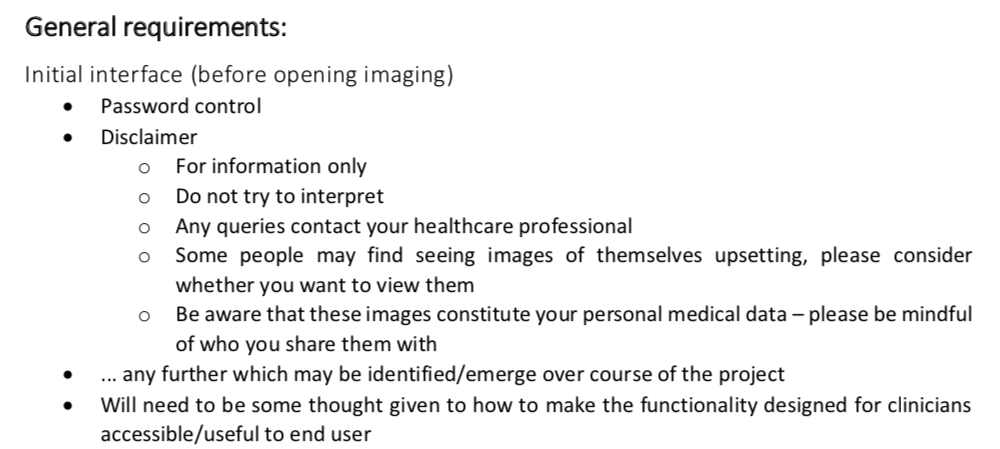
\includegraphics[width = 0.95\hsize]{./figures/GeneralSpec1}
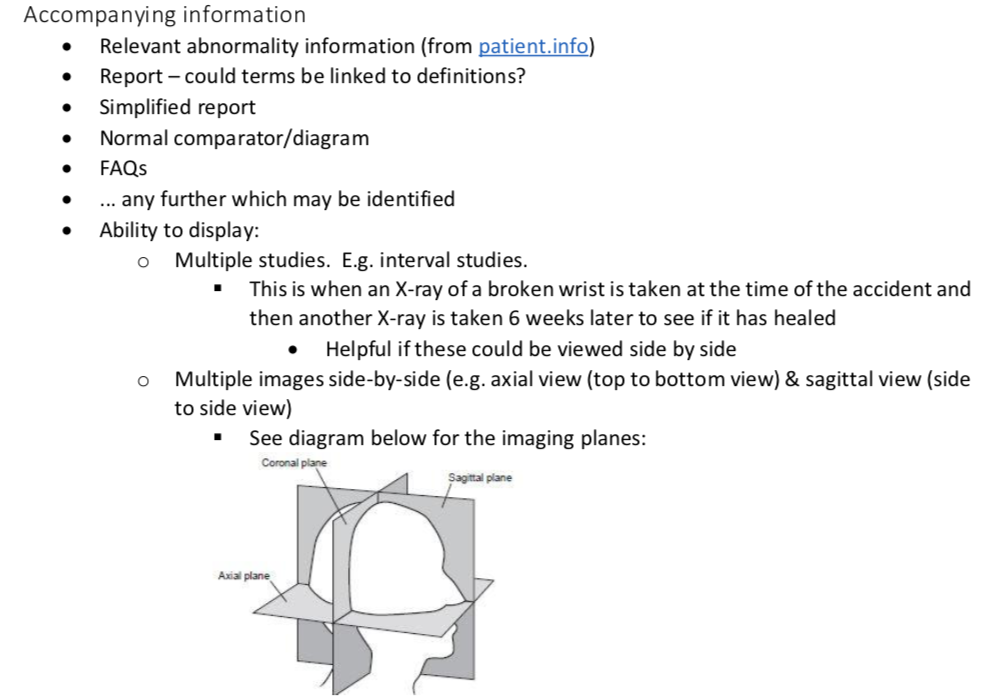
\includegraphics[width = 0.95\hsize]{./figures/GeneralSpec2}
\end{figure}



\clearpage

\begin{figure}[ht]
\centering
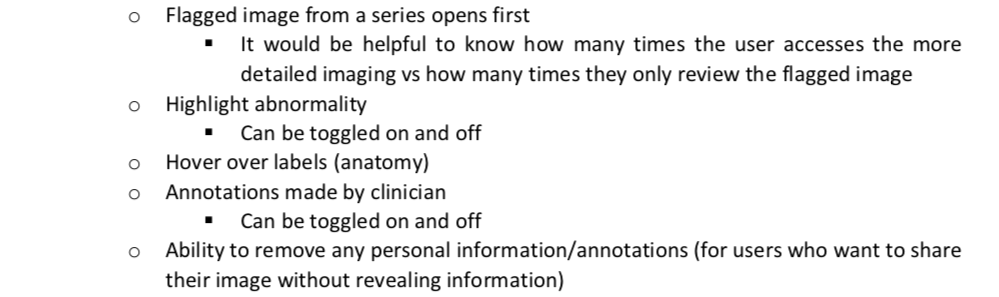
\includegraphics[width = 0.95\hsize]{./figures/GeneralSpec3}
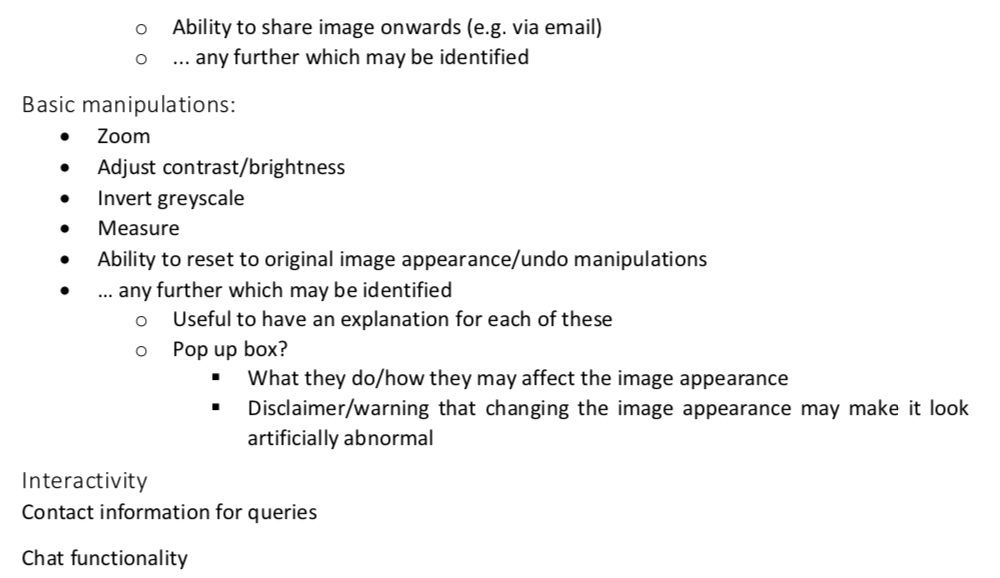
\includegraphics[width = 0.95\hsize]{./figures/GeneralSpec4}
\end{figure}

\clearpage

\subsection {Appendix 2 - Imaging Specification}

\begin{figure}[ht]
\centering
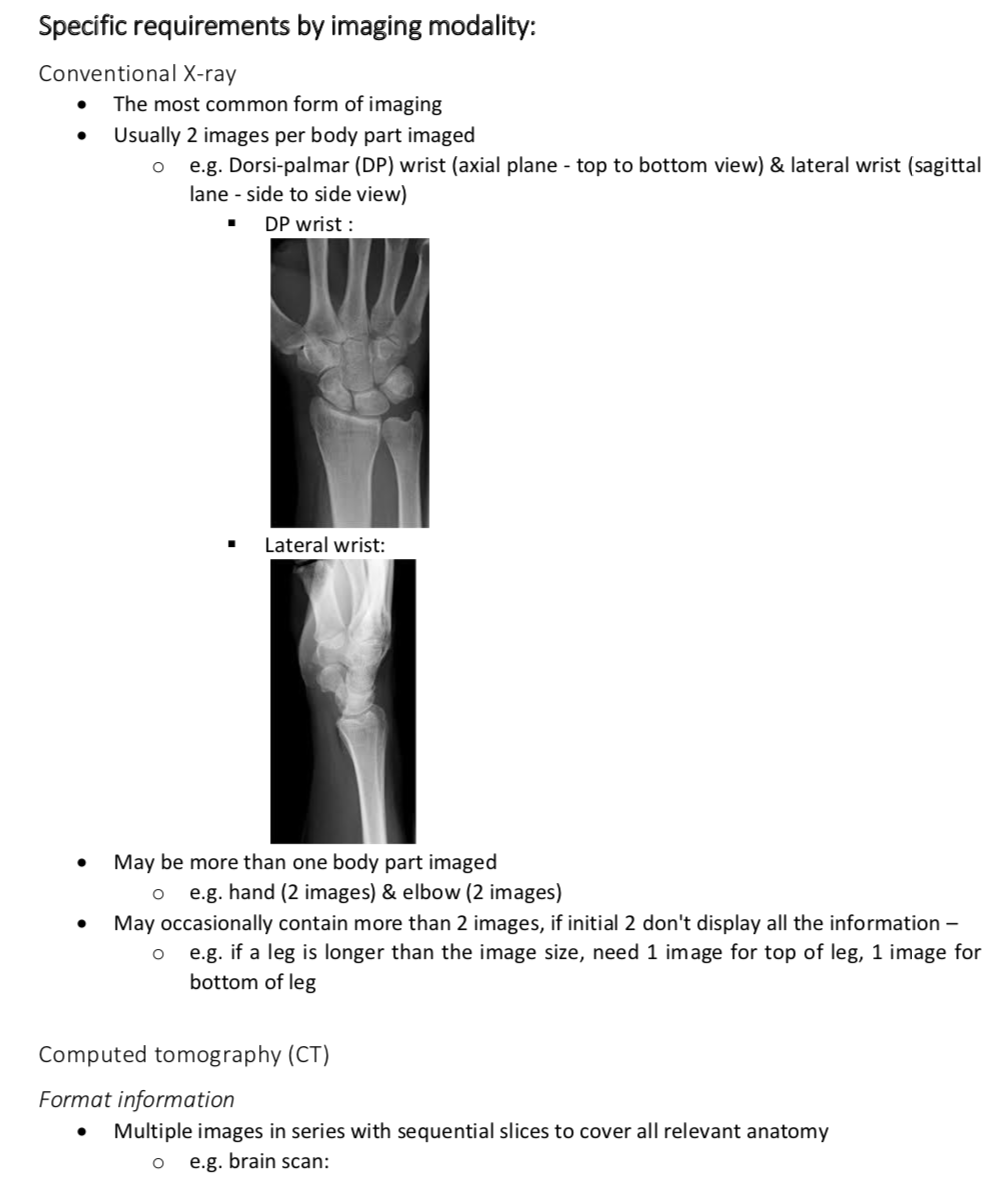
\includegraphics[width = 0.95\hsize]{./figures/ImagingSpec1}
\end{figure}
\clearpage

\begin{figure}[ht]
\centering
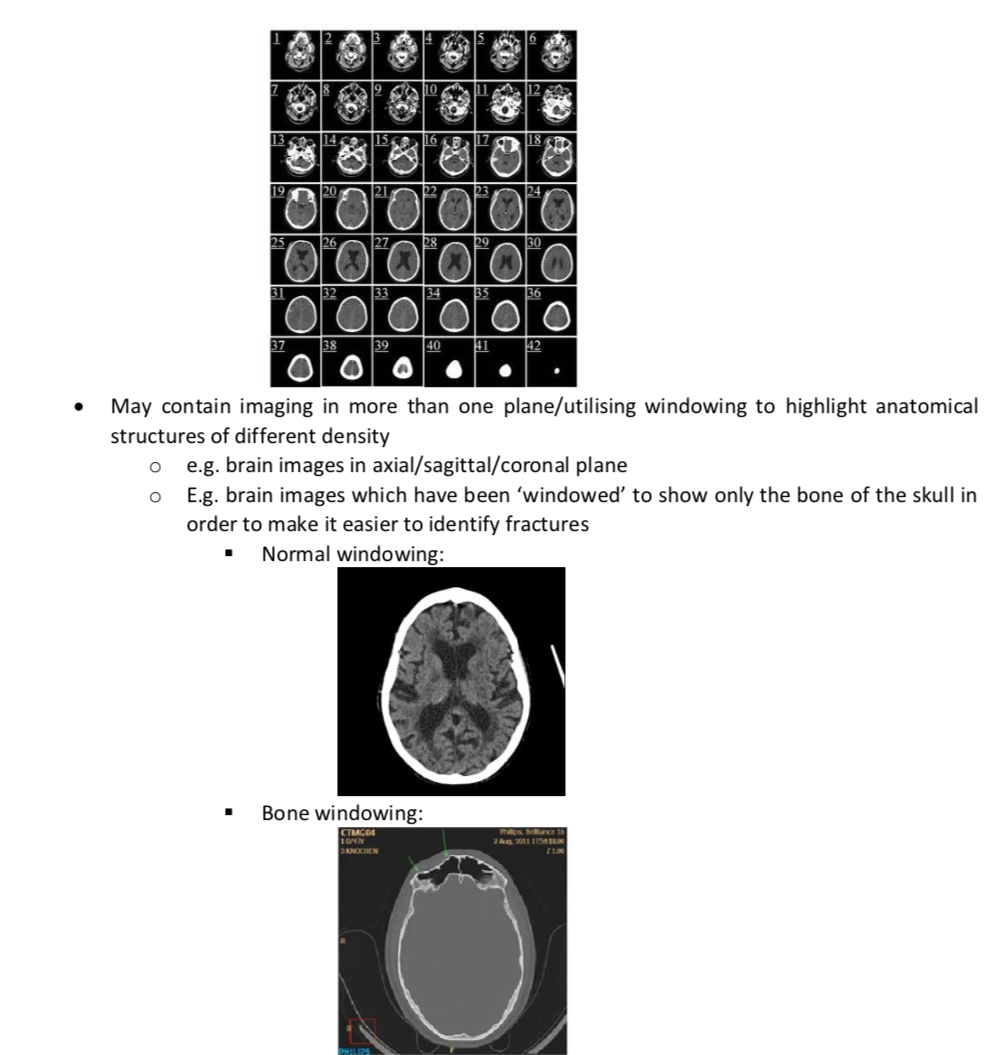
\includegraphics[width = 0.95\hsize]{./figures/ImagingSpec2}
\end{figure}
\clearpage

\begin{figure}[ht]
\centering
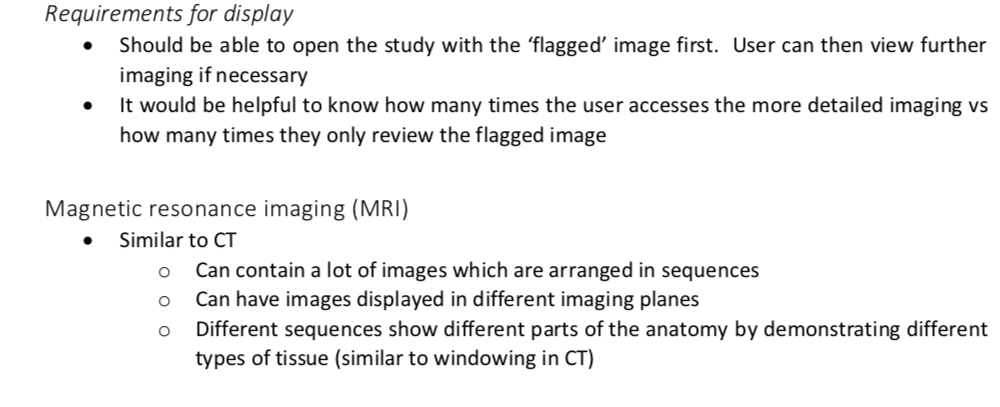
\includegraphics[width = 0.95\hsize]{./figures/ImagingSpec3}
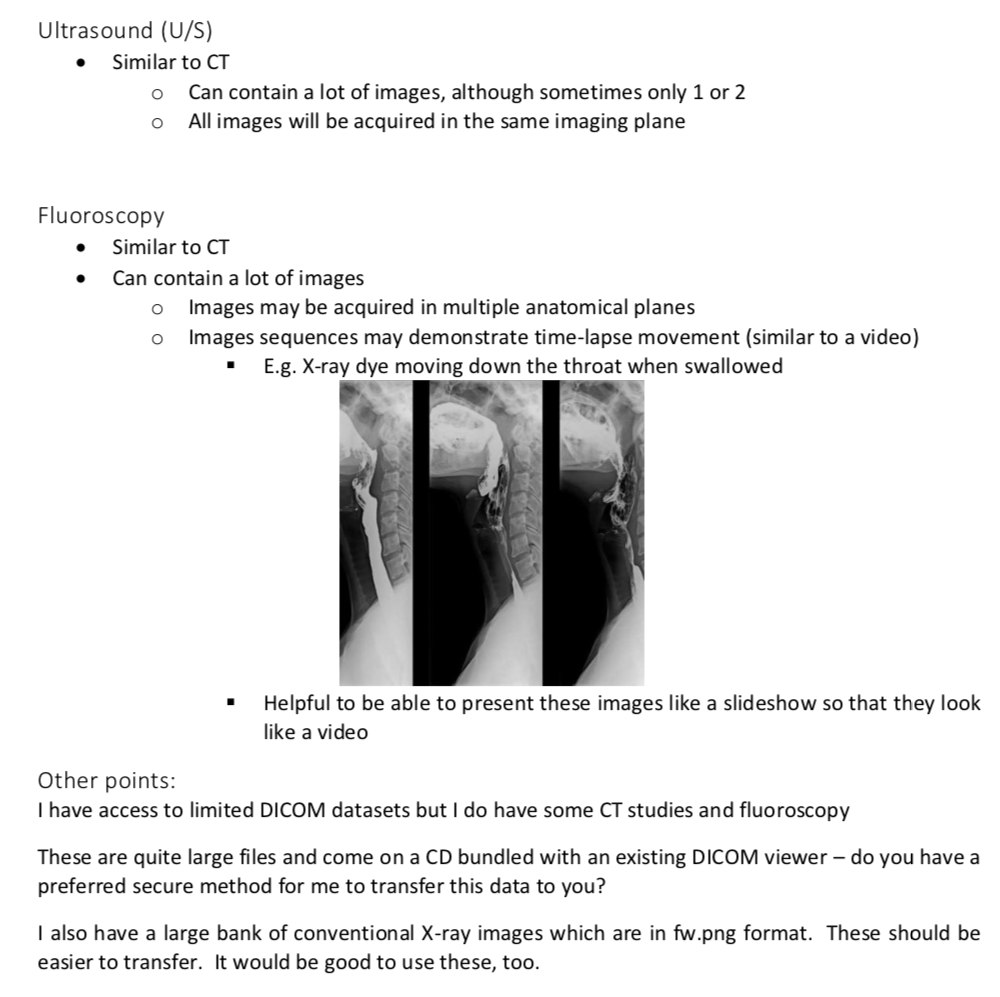
\includegraphics[width = 0.95\hsize]{./figures/ImagingSpec4}
\end{figure}
\clearpage



%% bibliography
\printbibliography


\end{document}
